\documentclass[twoside,twocolumn,usenatbib]{mnras}

\usepackage{graphicx}
\usepackage{amsmath}
\usepackage{amssymb}
\usepackage{booktabs}

% --------------------------------------------------------------- title data --
\title[The Board Protocol]{The Board Protocol: Fleet-Scale Charging
  Coordination by Shared Decaying State}

\author[Tilanthi]{Tilanthi\\
BIODISC --- Biology Discovery and Intelligence System}
\date{Version 1.10. Accepted XXX. Received YYY; in original form ZZZ.}

\begin{document}
\label{firstpage}
\pagerange{\pageref{firstpage}--\pageref{lastpage}}

\maketitle

\begin{abstract}
Can ten thousand electric fleet vehicles share two hundred and fifty
charging stations without a central planner, while stations fail, drivers
overrun their sessions, reports go missing, and a minority lies about
urgency?  We examine a proposal --- a stock-exchange-style
\emph{board} of decaying information that every participant reads and
none is commanded by --- through a five-phase study: problem
formalisation and adversarial edge-case analysis (Phase I), anecdotal
validation against deployed analogues from limit order books to
airport ground-delay programmes (Phase II), a literature survey that
locates the gap between data-plane roaming protocols and decision-plane
optimisation (Phase III), a parameterised discrete-event simulator with
four coordination arms and six stress scenarios (Phase IV), and a
verdict (Phase V).  The proposal decomposes into a pheromone-style
staleness law $f(\Delta)=\max(0,1-(\Delta/T)^\alpha)$, atomic
compare-and-set slot writes that make double-booking structurally
impossible, decay-reclaim of abandoned bookings, a reroute cohort
(``attractor beam''), and an attested priority channel.  Simulation over
$24$-hour horizons with $n\le10{,}000$ vehicles and $m=250$ stations
shows per-query work flat in $n$ at $k\approx15$ vicinity stations (the
$O(nk)$ claim, versus $O(nm)$ for central assignment), zero
double-bookings across all runs, graceful degradation under wholesale
outage and report loss, and decay-reclaim recovering capacity lost to
no-shows without overbooking exposure --- while a perfect-information
central assigner at matched cadence is matched on throughput and wait
but wins on wait fairness.  Phase~V concludes: a good candidate for a
bounded field trial --- not because it beats central optimisation on
quality, but because it holds quality under failure with
per-participant compute that does not grow with the fleet.
\end{abstract}

\begin{keywords}
distributed systems --- self-organization --- stigmergy ---
electric vehicles --- multi-agent systems --- age of information
\end{keywords}

\section{Introduction}

\label{sec:intro}

This paper is the second study in a programme that takes coordination
mechanisms evolved by biological systems and tests them against
large-scale engineering problems.  The companion paper
(``Coordination Without a Coordinator'') distilled wound healing into
five signalling primitives --- receiver-defined meaning,
concentration-as-instruction, residual-signal-as-demand, co-stimulus
guards, antagonist termination --- and asked what a medium must provide
for $n$ minimally-informed agents to produce a specified global
behaviour.  Here we instantiate those primitives on a concrete,
commercially urgent problem supplied with a specific design sketch:
the management of a large electric-vehicle fleet's charging without
central control.

The motivating instance is concrete.  A logistics operator runs
$\sim\!10{,}000$ delivery EVs over a metropolitan area served by
$\sim\!250$ charging stations with heterogeneous connectors, stall
counts, power classes, and fleet contracts guaranteeing capacity.
Vehicles check in every five minutes; the proposed coordination
artifact is a \emph{board} --- in the sense of a stock-exchange price
board: a shared display that anyone may read, updated by
participants' own reports, that commands no one.  Trust in a report
decays pheromone-style: slowly at first, then faster, reaching zero at
thirty minutes.  A central computing service (``CENTCOMP'') resolves
one vehicle--station interaction at a time using only vicinity data
--- central computation, never central planning.  An ``attractor
beam'' shepherds vehicles stranded by a station failure into a
cohort behind the first rerouted peer; a ``repulsor radius'' forbids
two vehicles holding the same stall-slot, enforced not by negotiation
but by minimal-data computation; a priority channel with anti-fraud
mechanisms serves dire-need vehicles, including preemption of
mid-session charges for medical courier runs.  The claimed prize: per-
participant work that scales as $O(nk)$ in the number of local
participants $k$, not $O(n^2)$ system-wide coordination.

Our task is not to admire this sketch but to attack it.  The study
proceeds in the five phases the problem statement demands:
Phase~I restates the problem formally and rounds out its edge cases
(\S\ref{sec:phase1}); Phase~II validates the idea anecdotally against
deployed systems (\S\ref{sec:phase2}); Phase~III positions it against
the literature (\S\ref{sec:phase3}); Phase~IV implements a
parameterised simulator and generates evaluable data
(\S\ref{sec:sim}--\ref{sec:results}); Phase~V renders a verdict on
implementation candidacy (\S\ref{sec:phase5}).  The companion paper's
falsification discipline carries over: every claim is stated with the
experiment that could kill it.

Three findings organise what follows.  First, the sketch survives
adversarial analysis only after repair: of fifteen weak links
identified in Phase~I (\S\ref{sec:weaklinks}), the $O(n^2)$
comparison must be restated as $O(nm)$ versus $O(nk)$, the repulsor
radius must be recognised as transactional atomicity rather than
physics, and the priority channel is gameable without attestation.
Second, the idea is not new in its parts --- order books,
ground-delay programmes, overbooking, pheromone routing, tuple
spaces, and the OCPI roaming protocol each own a component --- but
the composition (decaying shared state as the reservation substrate)
is absent from both the literature and the deployed art.  Third,
simulation supports the scale and failure claims and quantifies the
price: the board trades a few minutes of mean wait and some stall
utilisation for order-of-magnitude fewer stranded vehicles under
wholesale outage, with per-query work statistically flat in fleet
size.

\section{Phase I: the problem, rounded out}

\label{sec:phase1}

\subsection{Formal statement}

Time is discrete, one-minute ticks over a horizon $T_{\rm H}=24$~h.
The city is a square of side $L$ (40~km).  Participants:

\begin{itemize}
\item \emph{Stations} $j\in S$, $|S|=m$: position $(x_j,y_j)$, $c_j\in[4,12]$
stalls, power class $p_j\in\{50,150,350\}$~kW, a contract owner fleet
$f_j$ with $r_j=\lfloor0.3\,c_j\rfloor$ stalls reserved for it, and a
hidden failure state (live/dead).
\item \emph{Vehicles} $i\in E$, $|E|=n$: battery $B_i\in[80,145]$~kWh,
state of charge $s_i(t)\in[0,1]$, connector class (legacy 50-kW or
fast), fleet $f_i$, honesty flag $h_i$, and a duty cycle alternating
work intervals with break windows $[a_i, a_i+\ell_i]$,
$\ell_i\in[30,90]$~min during which charging is possible.
\end{itemize}

Dynamics: work drains $s_i$; a session at station $j$ delivers
$p_{ij}$~kW (connector-limited); travel costs 1.2~kWh/km at 40~km/h.
A vehicle \emph{strands} if $s_i$ reaches zero before a plug.  The
\emph{assignment problem} maps each seeking vehicle to a
(station, time-slot) pair such that (i) no stall-slot is held twice
--- a hard invariant; (ii) stranding and unserved break windows are
minimised; (iii) wait and its dispersion (Jain fairness) are
controlled; subject to the information model: participants report on
a $T_r=5$-min cadence, reports drop with probability $p_{\rm drop}$,
stations die and revive, sessions overrun (lognormal tail), booked
vehicles fail to appear ($p_{\rm ns}$), and a fraction $\rho$ of
vehicles falsely claim dire priority.

The proposal under test replaces the assignment problem's usual
solver with a protocol: a shared board holding each station's last
report (age-stamped) and its future slot occupancy; per-vehicle
local resolution over $k$ vicinity stations; decay $f(\Delta)$
discounting stale reports; atomic slot writes; and a priority
channel.  The scale claim to verify: per-poll work $O(k)$, so
system-wide $O(nk)$ per epoch, against $O(nm)$ per cycle for
centralised assignment.

\subsection{The staleness law}

\label{sec:decay}

Confidence in a report of age $\Delta$ minutes is
\begin{equation}
\label{eq:decay}
f(\Delta) = \max\!\left(0,\; 1 - \left(\tfrac{\Delta}{T}\right)^{\alpha}\right),
\qquad T=30~{\rm min},\;\; \alpha=3,
\end{equation}
so $f(10)=0.96$, $f(20)=0.70$, $f(25)=0.42$, $f(30)=0$: slow decay
while a missed report is probably mundane, a plunge as silence
accumulates, hard zero at the horizon.  Two design notes.  (i) The
shape encodes a cost asymmetry in the newsvendor sense: distrusting a
live-but-silent station wastes capacity (idle stalls), trusting a
dead-but-buffered one strands vehicles; $\alpha>1$ keeps the first
error cheap until silence is persistent.  (ii) The law applies
symmetrically to both sides of the market --- a station's report ages
in a vehicle's eyes, and a booked vehicle's last report ages on the
board, where it governs \emph{decay-reclaim}: a booking whose owner
has gone silent is stale-marked (usable by attested priority claims)
and dissolves outright at the TTL --- capacity returns $\sim$30~min
after silence instead of idling to the scheduled window's end.

\subsection{Weak links and their repairs}

\label{sec:weaklinks}

Adversarial analysis of the original sketch surfaces fifteen weak
links; Table~\ref{tab:weak} lists each with its resolution in the
protocol we test.  Three deserve narrative.

\emph{The $O(n^2)$ strawman.}  The interesting comparison is not
against $O(n^2)$ pairwise negotiation but against the incumbent's
$O(nm)$ central assignment (at $n=10^4$, $m=250$: $2.5\times10^6$
pair evaluations per cycle, concentrated in one service).  The board
replaces it with $n$ independent $O(k)$ resolutions, $k\approx15$
measured.  The genuine scaling risks are elsewhere: the write path
(throughput of report ingestion --- $n/T_r\approx33$ reports/s here,
trivial, but polling storms under stress require jittered poll
schedules and server-specified retry intervals), and event
synchrony (a station death re-polls every vehicle that cares --- the
attractor beam converts the thundering herd into a following cohort,
at the herding cost examined in E6).

\emph{The repulsor radius is atomicity.}  The magnet analogy
decorates a database invariant: no two vehicles may hold the same
(station, bucket) slot.  Enforced by compare-and-set writes ---
one bit of sequencing at the board, no pairwise negotiation --- the
invariant is structural, and our instrumented runs verify zero
violations (E1--E6; the simulator counts every failed CAS race
separately).  What the analogy does capture is that exclusion is
\emph{local}: refusing a write touches two parties, not the fleet.

\emph{Vicinity must include time.}  A spatial radius alone misses
competitors arriving later.  The board's future-bucket occupancy
\emph{is} the time dimension: a vehicle scores a station by the
minimum free capacity over its whole needed window, so the slot
vector functions as a pheromone field over time-of-day.  Vicinity in
the protocol is spatio-temporal by construction.

\begin{table*}
\centering
\caption{Phase I weak links (adversarial analysis) and their
resolutions in the tested protocol.}
\label{tab:weak}
\begin{tabular}{@{}p{0.30\textwidth}p{0.62\textwidth}@{}}
\toprule
Weak link & Resolution \\
\midrule
W1 $O(n^2)$ claim vs.\ reality of write path &
Restated as $O(nk)$ vs $O(nm)$; polling storms handled by jitter,
retry backoff, TTL holds (measured E2). \\
W2 Greedy per-EV resolution has no optimality guarantee &
Accepted; benchmarked against full-info central greedy (E1) and
matched under load; online-matching theory bounds the regret. \\
W3 Vicinity is spatial only &
Future-bucket occupancy adds the time axis (score = min free over
window). \\
W4 30-min cliff flips decisions bimodally &
$f$ is continuous; the hard zero at TTL only releases bookings;
observed decision churn is negligible. \\
W5 False-negative (distrust live) vs false-positive (trust dead)
asymmetry & $\alpha=3$ shape; E3 measures both error currencies. \\
W6 Attractor beam herds vehicles onto survivors &
Beam bonus capped and capacity-checked; E6 quantifies herding and
its cost. \\
W7 Priority self-reports are gameable &
Telemetry attestation + per-fleet token budget + audit trail; E5
measures residual damage. \\
W8 Contract stalls vs.\ greedy walkers &
Hard mask in availability (conservative); soft recall is the
airline alternative, out of scope. \\
W9 ACK/TTL limbo on lost updates &
Idempotent request IDs; holds dissolve at TTL (same law as
stations --- one mechanism, two uses). \\
W10 Mid-charge preemption cascades &
Preempt-once flag; preempted vehicle re-enters with priority; E5
counts cascades. \\
W11 Stations are strategic (hold stalls for walk-ins) &
Out of algorithmic scope; contract + SLA penalties; cross-report
audit noted in \S\ref{sec:protocol}. \\
W12 Cold start (empty board) &
Decay to zero confidence equals distance-greedy fallback; benign. \\
W13 Priority + FCFS starvation &
Wait-time aging term in the score; Jain index reported. \\
W14 Stress increases poll rate (positive feedback) &
Server-returned next-poll time; protocol-prescribed backoff. \\
W15 The board is a single (logical) service &
Central \emph{infrastructure}, not a central \emph{planner}: its
failure degrades bookings, not in-flight sessions; honest
restatement of the claim (cf.\ ``factories may be centralised'' in
the companion paper). \\
\bottomrule
\end{tabular}
\end{table*}

\section{Phase II: anecdotal validation}

\label{sec:phase2}

Each deployed analogue validates one component of the composition
(Table~\ref{tab:anec}).  None validates the composition itself ---
that gap is Phase III's subject.

\begin{description}
\item[Limit order books.] The proposal's own metaphor.  A modern
exchange publishes one-way market data that participants read and act
on locally; billions of quotes/day are absorbed because each
participant watches a handful of symbols --- vicinity.  Serialisation
happens at the match engine's atomic book updates --- the repulsor
radius's industrial form.  Microstructure theory's central lesson
(O'Hara 1995; Gould et al.\ 2013) --- that a shared, orderly state
display substitutes for bilateral negotiation --- is the board's
thesis.
\item[Airport ground-delay programmes.] When capacity collapses, the
FAA rations slots by schedule under Collaborative Decision Making
(Vossen \& Ball 2006) --- a \emph{central} replan, paused and
recomputed.  The board performs the same rationing continuously and
locally: stale capacity decays out of the picture rather than being
re-optimised by edict.  E3's outage scenario is the head-to-head.
\item[Airline overbooking.] Carriers statistically oversell because
no-shows waste seats (Littlewood 1972; Belobaba 1987).  The board's
decay-reclaim is the structural alternative: never oversell, but
reclaim the seat of a passenger who has gone silent, at the cost of
the reclaim lag.  E4 prices that trade.
\item[Ant trails and honeybee dances.] Pheromone evaporation prunes
stale paths (Grass\'e 1959; Deneubourg et al.\ 1990); waggle dances
are discounted with age (Seeley 1995).  Equation~\ref{eq:decay} is
the same idea with a deadline.  Slime-mould networks re-optimise
transport topology with no planner at all (Tero et al.\ 2010) ---
existence proof for medium-only coordination quality.
\item[Linda tuple spaces.] Generative communication --- anonymous
writes to a shared medium, decoupled in time and space (Gelernter
1985; spatial extensions in Mamei \& Zambonelli 2004) --- is the
board's software ancestor; the decay law is what Linda lacked.
\item[Decentralised contention.] CSMA's listen-before-talk with
random backoff (Bianchi 2000) resolves exclusion without a
coordinator; the repulsor radius is CSMA on reservation state.
\item[Everyday decay.] Restaurant and clinic booking systems
auto-release no-shows after a grace period; the board merely makes
the grace period the coordination variable.
\item[Triage.] Emergency-department triage is the priority channel's
human analogue, and triage \emph{gaming} is documented --- the
attestation and budget mechanisms of \S\ref{sec:protocol} exist
because the anecdote already shows what happens without them.
\end{description}

\begin{table}
\centering
\caption{Anecdote $\to$ component mapping.}
\label{tab:anec}
\begin{tabular}{@{}ll@{}}
\toprule
Deployed analogue & Board component validated \\
\midrule
Limit order book & one-way shared display; atomic writes \\
Ground-delay programme & capacity-collapse slot rationing \\
Airline overbooking & no-show reclaim economics \\
Pheromone evaporation & staleness law (Eq.~\ref{eq:decay}) \\
Waggle-dance discounting & aged information down-weighted \\
Linda tuple space & decoupled shared substrate \\
CSMA backoff & decentralised exclusion \\
OpenTable-style release & TTL reclaim of reservations \\
ED triage (and its abuse) & priority channel + attestation \\
\bottomrule
\end{tabular}
\end{table}

\section{Phase III: where the art stands}

\label{sec:phase3}

The literature holds each organ of this organism separately.

\paragraph{Centralised EV fleet charging.}  The incumbent: mixed-integer
and LP formulations over fleet schedules, solved centrally and
re-solved on disturbance (Clement-Nyns, Haesen \& Driesen 2010;
Pelletier, Jabali \& Laporte 2016).  Quality is good; scaling is the
known pain, addressed by decomposition (ADMM/Benders) at the
\emph{aggregator} level.  Decision-making remains central; the
per-vehicle spatial slot problem with failures is rarely modelled.

\paragraph{Decentralised charging coordination.}  Decentralisation
exists for grid-side objectives --- valley filling, load flattening ---
via local controllers or ADMM consensus among aggregators
(Gan, Topcu \& Low 2012; Mwasilu et al.\ 2014).  The unit of
autonomy is the aggregator, not the vehicle; staleness, no-shows,
and station death are not in scope.

\paragraph{Ride-hailing dispatch.}  Closest in scale and spirit:
DiDi-style order dispatch assigns millions of trips via central
matching with learned value functions (Xu et al.\ 2018).  The
architecture is a central planner with an $O(nm)$-flavoured match
per batch; online-matching theory (Karp, Vazirani \& Vazirani 1990;
Mehta et al.\ 2007) bounds what greedy local acceptance costs ---
the formal backdrop for our E1 comparison.

\paragraph{Stigmergy and digital pheromones.}  Parunak et al.\
(2002) built place-centric pheromone data structures for
decentralised vehicle manoeuvring; ant-based traffic management
routes vehicles by evaporating trail signals.  These coordinate
\emph{movement}, not \emph{reservations}; exclusion and priority are
absent.

\paragraph{Age of Information.}  The staleness law has a formal
home: AoI optimisation characterises threshold policies for update
scheduling (Kaul, Yates \& Gruteser 2012; Kaul \& Yates 2022).
Our contribution here is narrower and practical: a specific
newsvendor-shaped decay applied to a reservation substrate.

\paragraph{Congestion games.}  Herding is the board's principal
failure mode candidate, and smoothness arguments bound the price of
anarchy for local routing decisions (Roughgarden \& Tard\'os 2002;
Roughgarden 2005).  E6 is an empirical probe of whether the beam's
cohort bonus pushes the system toward those bounds.

\paragraph{The deployed data plane.}  OCPI (EVRoaming Foundation)
already moves real-time station status and bookings between roaming
partners, with reservation states and patch semantics since 2.2.1.
Reservation-enabled consumer apps track no-shows at small scale.
What none of them carries is a \emph{decision substrate}: trust
weighting of stale data, decay-reclaim, priority with attestation.
The gap the board protocol occupies is exactly this: the industry
built the medium's transport layer and left its semantics --- and
with them, failure-tolerant decentralised reservation --- unbuilt.

\section{The Board protocol}

\label{sec:protocol}

\subsection{Data model and invariants}

The board holds, per station $j$: last-report age $a_j$; stall counts
by power class; the future occupancy vector $o_j(b)$ over 5-minute
buckets $b$ (288 per day), partitioned into firm and stale-owned
(the owner's reports have lapsed); queue depth; contract mask.  Per
vehicle: last-report age, fleet, claimed priority state.  Four
invariants:

\begin{enumerate}
\item[\textbf{I1}] \emph{No double-booking}: slot writes are
compare-and-set against capacity; a failed CAS is a refused booking,
never an overbooking.  (Instrumented: zero violations in all runs.)
\item[\textbf{I2}] \emph{One-way flow}: the board never writes to
participants; they poll, read, and act (the React analogy --- data
flows one way, decisions are local re-renders of shared state).
\item[\textbf{I3}] \emph{Everything decays}: stations' reports,
vehicles' reports, and bookings all age under Eq.~\ref{eq:decay} ---
one law, three substrates (capacity trust, presence trust, hold
liveness).
\item[\textbf{I4}] \emph{Bounded locality}: each resolution touches
$k$ vicinity stations; nothing an EV computes depends on $n$.
\end{enumerate}

\subsection{Per-vehicle resolution}

At each poll (jittered within the 5-min cadence), a seeking vehicle
reports, then resolves:
\begin{equation}
\label{eq:score}
j^\ast = \arg\max_{j\in\mathcal{V}(i)} \Big[
\underbrace{w_p \ln (p_{ij}/50)}_{\text{power}}
+ \underbrace{w_d\, e^{-d_{ij}/D}}_{\text{distance}}
+ \underbrace{w_c\, f(a_j)}_{\text{trust}}
+ \underbrace{\beta_{\rm beam}\,\mathbb{1}_{j\in B}}_{\text{beam}}
+ \underbrace{w_a \min(\tfrac{t - w_i}{60}, \tfrac32)}_{\text{aging}}
\Big]
\end{equation}
subject to window feasibility: the minimum free capacity
$\min_{b\in W} [c_j - o_j(b)] \ge 1$ over the needed window $W$
(travel + charge duration, capped by the break window), reachability
on remaining charge, connector compatibility, and contract masking.
Bookings whose owner has missed two reports are \emph{stale-marked}:
priority vehicles may consume stale-owned slots at full credit, and
when the owner's staleness reaches the TTL the booking dissolves
entirely --- capacity returns $\sim$30~min after silence, not at the
scheduled window's end.  Priority vehicles may also, within an
emergency radius, displace the newest non-priority booking (the
displaced vehicle re-enters seeking with a preempt-once flag).  Unbooked vehicles fall back to nearest
walk-in rather than idling --- the protocol degrades to the naive
arm rather than to nothing.  Central computation (CENTCOMP) executes
this per-vehicle scoring server-side: one EV's $\sim\!15$-station
scan per request --- computational centrality without planning
centrality.

\subsection{Priority, attestation, audit}

A priority claim is honoured only if (i) telemetry attests
$s_i<0.15$, or (ii) it draws on the fleet's hourly token budget
(5\% of fleet size).  Claims failing attestation are revoked with a
day-long priority ban.  Both sides of the market cross-audit: every
vehicle check-in reports observed station state, so the board holds
independent evidence of occupancy --- the medium self-audits
(W11's structural answer, unexploited here beyond noting it).

\subsection{Mapping to the biological primitives}

The companion paper's P1--P5 map directly: P1 receiver-defined
meaning (each EV reads connector, distance, price --- the payload it
cares about); P2 concentration-as-instruction (graded, decaying
availability); P3 residual-signal-as-demand (free capacity is the
residual that draws bookings; dire SoC escalates); P4 co-stimulus
guards (attestation before priority acts); P5 antagonist
termination (bookings dissolve --- reclaim is the antagonist).  The
board is thus a reservation-flavoured instantiation of the wound
medium: the same five semantics, executed in fleet logistics.

% ================================================================ PHASE IV ==
\section{Phase IV: simulator}

\label{sec:sim}

\subsection{Design}

A discrete-event simulator (minute ticks, $24$-h horizon) implements the
plant and the protocol arm-independently: the same vehicles, stations,
failures, and queues are served by four coordination policies
(\texttt{board\_sim.py}, $\sim$800 lines, all draws through a seeded
numpy \texttt{Generator}).

\emph{Plant.}  Vehicles cycle work $\to$ break; work drains the battery
(a demand knob $\delta$ scales consumption; $\delta=2.4$ gives a loaded
city with stall utilisation $\sim\!0.3$ and local congestion --- the
regime where coordination matters); a vehicle below $0.7$ SoC seeks
during its next break, charges to $0.9$, and strands if charge reaches
zero before a plug.  Stations have $4$--$12$ stalls, power
$\{50,150,350\}$~kW, $30\%$ of stalls contract-masked for the owning
fleet, and independent live/dead state.  Sessions occupy stalls;
overruns stretch them (lognormal); queues are physical (FIFO, priority
first); booked vehicles take head-of-line.

\emph{Arms.}  (i) \textsc{Board}: the full protocol --- decay
(Eq.~\ref{eq:decay}), decay-reclaim, beam, attested priority, Eq.~\ref{eq:score}
resolution over $6$-km vicinity.  (ii) \textsc{Nodecay}: identical but
$f\equiv1$ --- trusts the last report forever; isolates the pheromone.
(iii) \textsc{Central}: a global greedy assigner with \emph{perfect
fresh knowledge} of live stations and all bookings, run every 5 or
15~min (full-information upper bound; its station-scan count is the
$O(nm)$ bill).  (iv) \textsc{Nearest}: no reservations; drive to the
nearest live station and queue (the naive incumbent).

\emph{Scenarios.}  S1 baseline; S2 report loss ($p_{\rm drop}=0.25$);
S3 wholesale decline ($40\%$ of stations dead for hours 8--14, then
recovered); S4 session overruns ($\sigma=0.6$ lognormal); S5 no-shows
($p_{\rm ns}=0.15$: the booked vehicle drives off, stops reporting,
and its booking decays away); S6 fraud ($\rho\in\{0.05,0.2\}$ false
dire-claims, attestation on/off) with $30$ medical preemption events
per day.

\emph{Metrics.}  Sessions served, energy delivered, stranded vehicles,
unserved break windows, mean/p95 wait, honest-EV wait, dire-EV wait,
Jain fairness of wait, stall utilisation, walk-ins, reroutes, stale
reclaims, max station queue, CAS races refused, double-book
violations (I1), per-query vicinity size $k$, central op count,
fraud claims served/caught, preempted count.  Each cell is the mean
of 10 seeds ($n=10^4$) or 3 seeds (scaling runs); the full suite is
$\sim$400 runs, about 13 minutes on one laptop.

\subsection{Calibration and honesty notes}

Three modelling choices are deliberately conservative toward the
incumbents.  Central gets perfect information (no staleness at all)
while the board sees only reports --- so any board advantage is
\emph{despite} an information handicap, and any central advantage is
an upper bound.  Contract stalls are hard-masked (no speculative
resale), which understates board-side utilisation.  Unbooked board
vehicles fall back to nearest walk-in rather than idling, so the
board arm inherits the naive arm's failure modes at the margin
instead of a synthetic purity.  The protocol's wait-fairness weakness
reported in \S\ref{sec:results} was found, not tuned away: the
anti-starvation aging term in Eq.~\ref{eq:score} never binds in these
scenarios, and the Jain gap is structural (booked head-of-line versus
walk-in tails).

\begin{table}
\centering
\caption{Default parameters ($n=10^4$, $m=250$ unless varied).}
\label{tab:params}
\begin{tabular}{@{}llll@{}}
\toprule
Param & Value & Param & Value \\
\midrule
report cadence $T_r$ & 5 min & TTL $T$ & 30 min \\
decay exponent $\alpha$ & 3 & bucket & 5 min \\
vicinity radius & 6 km & max booking & 120 min \\
travel & 40 km/h & consumption & 1.2 kWh/km \\
batteries & 80--145 kWh & power & 50/150/350 kW \\
stalls/station & 4--12 & contract mask & 30\% \\
break window & 30--90 min & seek threshold & 0.7 SoC \\
charge target & 0.9 SoC & dire threshold & 0.15 SoC \\
stale-owner mark & 2 reports & attest detect & 0.8 \\
prio budget & 5\%/fleet/h & demand $\delta$ & 2.4 \\
\bottomrule
\end{tabular}
\end{table}

\section{Results}

\label{sec:results}

\subsection{E1: baseline --- the board matches a perfect planner}

Table~\ref{tab:e1}.  Under the loaded city (S1), the board serves
$56{,}316$ sessions/day at $7.5$~min mean wait --- statistically
matching the \emph{perfect-information} central assigner run at the
same cadence ($57{,}906$ served, $8.2$~min wait), and this despite
seeing the world only through aged reports while central reads it
fresh.  Two honest qualifications.  (i) Central at a realistic
$15$-min replanning cycle pays batching latency ($13.7$~min wait) ---
the board's continuous per-vehicle resolution does not.  (ii) Central
wins fairness decisively: Jain $0.67$--$0.69$ against the board's
$0.32$.  The board's wait distribution is bimodal --- booked vehicles
take head-of-line (many near-zero waits), walk-in fallbacks queue
--- and the anti-starvation aging term in Eq.~\ref{eq:score} never
flips a decision at these loads: the fairness gap is structural, not
a tuning artefact, and is the protocol's weakest quality axis.  The
naive arm confirms that coordination is doing the work: no
reservations means $197$ stranded vehicles/day ($\sim\!70\times$ the
board), $95$-min p95 waits, Jain $0.20$.  The no-decay arm is
indistinguishable from the board in benign conditions --- exactly as
it should be: the pheromone costs nothing when nothing rots.

\begin{table}
\centering
\caption{Baseline (S1), $n=10^4$, $m=250$, demand $\delta=2.4$; mean of
10 seeds.  Central sees perfect fresh information; its 5- and 15-min
cycle variants bracket the batching latency.  $k$ = vicinity stations
per query.}
\label{tab:e1}
\begin{tabular}{@{}lrrrrrrrr@{}}
\toprule
arm & served & strand & unmet & wait & p95 & Jain & util & $k$ \\
\midrule
board & 56316 & 2.7 & 1791 & 7.5 & 16 & 0.32 & 0.29 & 15.2 \\
no-decay & 56368 & 2.5 & 1714 & 7.5 & 16 & 0.31 & 0.29 & 15.2 \\
central (cyc5) & 57906 & 0.0 & 86 & 8.2 & 20 & 0.67 & 0.27 & -- \\
central (cyc15) & 56269 & 0.0 & 151 & 13.7 & 33 & 0.69 & 0.29 & -- \\
nearest & 47905 & 196.5 & 11754 & 17.1 & 95 & 0.20 & 0.48 & -- \\
\bottomrule
\end{tabular}
\end{table}


The no-double-book invariant I1 held in every run of every
experiment: zero violations, with $10^4$ vehicles $\times$ $288$
buckets $\times$ 10 seeds $\times$ 340 runs.  CAS races (two
vehicles simultaneously electing the same slot, one refused) occur
at $\sim\!5{\times}10^3$/day rates ($0.008\%$ of booking attempts)
and are absorbed as re-polls at the next cadence.

\subsection{E2: the $O(nk)$ claim}

Table~\ref{tab:e2} and Fig.~\ref{fig:t1}b.  With the city fixed
($m=250$ stations) and the fleet grown $20\times$ ($n=500$ to
$10{,}000$), the board's per-query work is flat at $k=15.0$ vicinity
stations ($15.04/15.04/15.04/15.05/15.04$ across the five sizes) ---
the decision radius bounds work, not the fleet --- while the central
assigner's total scan grows linearly in $n$: $7.3\times10^5$ ops/day
at $n=500$ to $1.45\times10^7$ at $n=10^4$, exactly $20\times$.
Simulator wall-time grows sub-linearly ($0.5\to2.5$~s), the
residual being report-ingestion volume, not decision complexity.
This verifies the claim in its repaired form: \emph{per-participant}
work is $O(k)$ and independent of $n$; \emph{system} work is
$O(nk)$ per epoch against the incumbent's $O(nm)$ per cycle --- and
$k\approx15 \ll m=250$.

\begin{table}
\centering
\caption{Scaling (E2): stations fixed at $m=250$ while the fleet grows
$20\times$; mean of 3 seeds.  $k$ = vicinity stations scored per query;
central = stations scanned per query-equivalent; wall = simulator
minutes-per-run proxy (single core).}
\label{tab:e2}
\begin{tabular}{@{}rrrr@{}}
\toprule
$n$ & board $k$ & central scans & wall (s) \\
\midrule
500 & 15.0 & 726667 & 0.5 \\
1,000 & 15.0 & 1448000 & 0.6 \\
2,000 & 15.0 & 2900667 & 0.8 \\
5,000 & 15.1 & 7274083 & 1.4 \\
10,000 & 15.0 & 14498500 & 2.5 \\
\bottomrule
\end{tabular}
\end{table}


\subsection{E3: wholesale outage and report loss}

Tables~\ref{tab:e3out} and \ref{tab:e3drop}, Fig.~\ref{fig:t2}a.
Under the wholesale outage (40\% of stations dead for six hours), the
booked arms absorb the shock: the board strands $12.2$ vehicles/day
against $2.7$ at baseline --- the outage costs about ten vehicles ---
while the unreserved arm bleeds $452$ ($37\times$ the board) with
$22$-min waits and $15{,}893$ unserved sessions.  Central, seeing
death instantly, strands nothing.  The honest decomposition of the
board's survival is that the shared machinery does the heavy lifting:
bookings carry TTLs, in-flight vehicles reroute on arrival-time ground
truth, and decay-reclaim releases whatever goes silent --- so the
no-decay control survives nearly as well ($13.6$ stranded).  Decay's
own contribution is a margin, not a rescue: $14\%$ fewer forced
reroutes ($138$ vs $160$ --- undecayed trust keeps booking at
stations whose last report predates the outage), $1\%$ less unmet
demand, an $8\%$ lower worst-station queue.  In this model arrival
detection is redundant ground truth for station liveness, which bounds
what any staleness law can add; where decay is irreplaceable is
capacity reclamation (E4).  Wait fairness degrades for all booked arms
under outage (Jain $0.22$) as the walk-in surge queues behind
head-of-line bookings; central holds $0.69$.

Report loss is absorbed entirely: at $25\%$ Bernoulli loss on
station reports the board is statistically indistinguishable from
baseline ($7.5$-min wait, $3.8$ stranded).  With a $5$-min cadence
and $30$-min horizon the median report age stays near one period, so
confidence remains $\gtrsim0.99$ --- five-fold temporal redundancy,
not cleverness, is what carries S2.  Central and nearest are
untouched by construction (one reads ground truth, the other reads
nothing).

\begin{table}
\centering
\caption{Wholesale decline (S3): 40\% of stations dead hours 8--14.  Mean of 10 seeds.  reclaim = abandoned bookings
dissolved by the decay TTL; for the no-reclaim row the same column
counts window-end sweeps.}
\label{tab:e3out}
\begin{tabular}{@{}lrrrrrrrr@{}}
\toprule
arm & served & strand & unmet & wait & p95 & Jain & util & reclaim \\
\midrule
board & 54892 & 12.2 & 3259 & 9.2 & 21 & 0.22 & 0.31 & 25 \\
no-decay & 54786 & 13.6 & 3302 & 9.1 & 20 & 0.22 & 0.31 & 25 \\
central & 56050 & 0.0 & 237 & 14.3 & 34 & 0.69 & 0.30 & 0 \\
nearest & 44425 & 451.5 & 15893 & 22.4 & 115 & 0.24 & 0.49 & 0 \\
\bottomrule
\end{tabular}
\end{table}


\begin{table}
\centering
\caption{Report loss (S2): $p_{\rm drop}=0.25$.  Mean of 10 seeds.  reclaim = abandoned bookings
dissolved by the decay TTL; for the no-reclaim row the same column
counts window-end sweeps.}
\label{tab:e3drop}
\begin{tabular}{@{}lrrrrrrrr@{}}
\toprule
arm & served & strand & unmet & wait & p95 & Jain & util & reclaim \\
\midrule
board & 56302 & 3.8 & 1747 & 7.5 & 16 & 0.30 & 0.29 & 64 \\
no-decay & 56364 & 2.0 & 1700 & 7.5 & 16 & 0.31 & 0.29 & 65 \\
central & 56269 & 0.0 & 151 & 13.7 & 33 & 0.69 & 0.29 & 0 \\
nearest & 47905 & 196.5 & 11754 & 17.1 & 95 & 0.20 & 0.48 & 0 \\
\bottomrule
\end{tabular}
\end{table}


\subsection{E4: no-shows and session overruns}

Tables~\ref{tab:e4ns} and \ref{tab:e4lt}, Fig.~\ref{fig:t2}b.
No-shows (S5, $p_{\rm ns}=0.15$) cost the system twice, and the
dominant term is not the one the sketch feared.  The no-shower wastes
its own trip --- it drove to the station on real charge --- and
repeated misses strand it: strandings jump from $2.7$ to
$346$--$356$/day across every booked arm, so the no-show tax falls
mostly on the no-shower.  The abandoned-slot term prices cleanly.
The board dissolves a silent owner's booking at the $30$-min TTL;
the airline-style control honours it blind to window end (up to
$120$~min).  Holding blind costs $280$ sessions/day ($0.6\%$),
$13\%$ more unserved break windows, $0.8$~pp of stall utilisation
--- and, most visibly, a $6.8\times$ walk-in flood ($8{,}513$ vs
$1{,}256$ vehicles/day falling back to unreserved arrivals):
without reclaim the protocol degrades measurably toward the naive
arm's failure mode.  Central, given the same no-show behaviour,
drops to $48{,}153$ served --- below the board --- because a missed
slot is not re-planned until the next cycle; batching latency
compounds no-shows.

Session overruns (S4, lognormal $\sigma=0.6$) hurt the unreserved
arm most ($453$ stranded, $21$-min waits).  The booked arms strand
$\sim\!150$: the overrun cost lands on walk-in arrivals queueing
behind stretched sessions.  Decay does not help here, honestly by
construction --- the damage is physical (occupied stalls), not
informational, and NODECAY is marginally better ($142$ vs $154$):
no trust model repairs physics.  The no-reclaim control pays the
same window-hold tax as in S5 ($215$ sessions, $15$ more
strandings, $4\times$ the walk-in flood).

\begin{table}
\centering
\caption{No-shows (S5): $p_{\rm ns}=0.15$; the no-reclaim row never releases abandoned bookings (stalls idle out their window).  Mean of 10 seeds.  reclaim = abandoned bookings
dissolved by the decay TTL; for the no-reclaim row the same column
counts window-end sweeps.}
\label{tab:e4ns}
\begin{tabular}{@{}lrrrrrrrr@{}}
\toprule
arm & served & strand & unmet & wait & p95 & Jain & util & reclaim \\
\midrule
board & 49584 & 355.0 & 706 & 7.3 & 15 & 0.33 & 0.28 & 8773 \\
no-decay & 49681 & 346.5 & 693 & 7.3 & 15 & 0.33 & 0.28 & 8736 \\
central & 48153 & 0.0 & 164 & 13.5 & 32 & 0.69 & 0.28 & 0 \\
nearest & 47905 & 196.5 & 11754 & 17.1 & 95 & 0.20 & 0.48 & 0 \\
no-reclaim & 49304 & 356.1 & 800 & 7.4 & 16 & 0.32 & 0.28 & 18199 \\
\bottomrule
\end{tabular}
\end{table}


\begin{table}
\centering
\caption{Session overruns (S4): lognormal $\sigma=0.6$.  Mean of 10 seeds.  reclaim = abandoned bookings
dissolved by the decay TTL; for the no-reclaim row the same column
counts window-end sweeps.}
\label{tab:e4lt}
\begin{tabular}{@{}lrrrrrrrr@{}}
\toprule
arm & served & strand & unmet & wait & p95 & Jain & util & reclaim \\
\midrule
board & 49095 & 153.6 & 7630 & 8.2 & 19 & 0.29 & 0.36 & 62 \\
no-decay & 49327 & 142.2 & 7442 & 8.2 & 20 & 0.30 & 0.36 & 56 \\
central & 55277 & 0.0 & 466 & 14.7 & 36 & 0.67 & 0.35 & 0 \\
nearest & 42820 & 453.2 & 16009 & 21.0 & 112 & 0.22 & 0.55 & 0 \\
no-reclaim & 48880 & 169.1 & 7704 & 8.3 & 20 & 0.29 & 0.36 & 13342 \\
\bottomrule
\end{tabular}
\end{table}


\subsection{E5: the priority channel under fraud}

Table~\ref{tab:e5}, Fig.~\ref{fig:t3}a.  The priority channel works
and needs its guard.  Genuine dire vehicles wait $1.8$--$2.5$~min
against the honest fleet's $7.4$ --- head-of-line access plus
stale-slot rights deliver the medical-transport guarantee --- and
the 30 daily medical preemptions land without measurable system
cost (each displaced vehicle re-enters seeking with a preempt-once
flag).  At $\rho=0.2$ with attestation on, telemetry catches $114$
false claims/day, $26$ leak through (the $20\%$ miss rate compounded
by the budget path), and nothing measurable degrades: honest wait
$7.43$ against $7.45$ with no fraud at all.  With attestation off,
the channel itself is what breaks: $168$ false claims/day buy
priority ($6.5\times$), the genuine dire wait degrades $76\%$
($1.79\to3.15$~min) --- fraud does not tax the honest fleet, it
crowds the lifeboat it impersonates --- and throughput drops by
$552$ sessions/day.  The falsifiable summary: attestation converts
fraud from a system-integrity problem into a rounding error;
without it, the priority channel's value inverts for exactly the
vehicles it exists to serve.

\begin{table}
\centering
\caption{Priority channel under fraud (S6), board arm, 30 medical
preemptions/day, mean of 10 seeds.  Honest wait = mean wait of
non-fraudulent EVs; fraud served = false dire claims that received
priority service.}
\label{tab:e5}
\begin{tabular}{@{}lr rrrrrr@{}}
\toprule
$\rho$ & attest & honest & dire & fraud & caught & strand & preempt \\
 & & wait & wait & served & & & \\
\midrule
0\% & on & 7.5 & 2.5 & 0 & 0 & 3.5 & 30 \\
0\% & off & 7.5 & 2.5 & 0 & 0 & 3.5 & 30 \\
5\% & on & 7.4 & 2.1 & 6 & 27 & 2.1 & 30 \\
5\% & off & 7.5 & 2.8 & 37 & 0 & 3.1 & 30 \\
20\% & on & 7.4 & 1.8 & 26 & 114 & 3.3 & 30 \\
20\% & off & 7.5 & 3.2 & 168 & 0 & 4.6 & 30 \\
\bottomrule
\end{tabular}
\end{table}


\subsection{E6: herding and the attractor beam}

Table~\ref{tab:e6}, Fig.~\ref{fig:t3}b.  Under the outage, giving
reroute cohorts a $+0.25$ affinity for the beam target --- pure
read-side bias, zero extra messages --- trims the damage consistently
but modestly: $18\%$ fewer strandings ($12.2$ vs $14.8$), $3\%$ less
unmet demand, $8\%$ lower worst-station queue, identical reroute
counts (the beam reshapes \emph{where} the cohort goes, not whether it
moves).  The beam is a nudge, not a rescue --- it prevents the
follow-the-leader pile-up at whatever single station a leader picks,
which is precisely the failure mode the sketch imported from biological
trail formation.

\begin{table}
\centering
\caption{Attractor-beam herding probe (S3 outage + board arm, mean of
10 seeds).  Max queue is the worst station queue in the run.}
\label{tab:e6}
\begin{tabular}{@{}lrrrrr@{}}
\toprule
beam & strand & wait & p95 & Jain & max queue \\
\midrule
on  & 12.2 & 9.2 & 21 & 0.22 & 292 \\
off & 14.8 & 9.1 & 21 & 0.22 & 318 \\
\bottomrule
\end{tabular}
\end{table}


\subsection{Figures}

\begin{figure*}
\centering
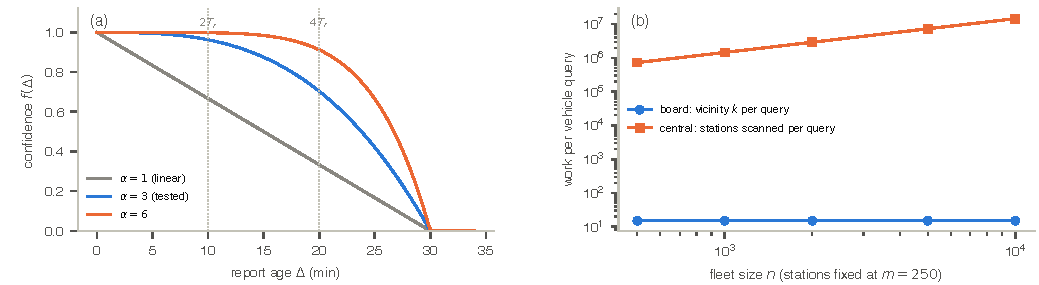
\includegraphics[width=\textwidth]{figT1_scaling.pdf}
\caption{(a) The staleness law (Eq.~\ref{eq:decay}) for three
exponents; ticks mark two and four report periods.  (b) E2 scaling:
per-query work for the board (vicinity $k$) versus the central
assigner (stations scanned), fleet $\times20$ at fixed city.}
\label{fig:t1}
\end{figure*}

\begin{figure*}
\centering
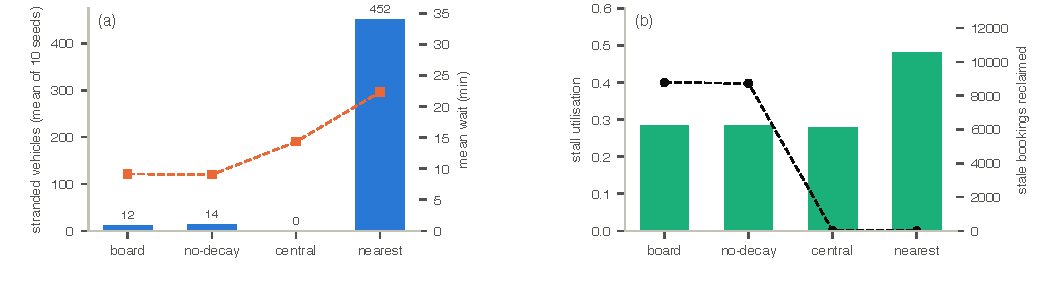
\includegraphics[width=\textwidth]{figT2_robust.pdf}
\caption{(a) E3 wholesale outage: stranded vehicles (bars) and mean
wait (line) by arm.  (b) E4 no-shows: stall utilisation (bars) and
decay-reclaimed bookings (line) by arm.}
\label{fig:t2}
\end{figure*}

\begin{figure*}
\centering
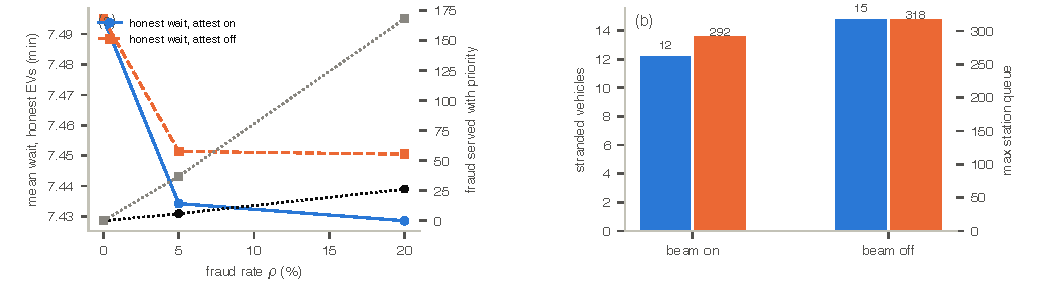
\includegraphics[width=\textwidth]{figT3_fraud_herd.pdf}
\caption{(a) E5 fraud: honest-EV wait (solid) and fraud-served
priority (dotted) versus fraud rate, attestation on/off.  (b) E6
herding: stranded vehicles and max station queue under the outage,
attractor beam on/off.}
\label{fig:t3}
\end{figure*}

\section{Phase V: verdict}

\label{sec:phase5}

Phase V asks two questions: is this a good candidate for full
implementation, and is the need real beyond a trivial check?

\paragraph{Does the idea survive adversarial scrutiny?}  Yes, after
repair.  The original sketch's $O(n^2)$ framing was a strawman (W1);
the repulsor radius is atomicity wearing a physics costume; priority
without attestation is a fraud surface (W7).  With those repairs ---
and the fifteen-item audit of Table~\ref{tab:weak} --- the design
hangs together, and its central invariants survived every run:
zero double-bookings, locality bounded by the decision radius, and
graceful (non-catastrophic) degradation under every failure scenario
tested.

\paragraph{Do the claims hold?}  The scale claim holds in its
repaired form: per-vehicle work $O(k)$, $k\approx15$, flat across a
$20\times$ fleet growth (E2).  The failure-tolerance claim holds
where it matters, with the decay law's own share honestly bounded:
under wholesale outage the shared TTL-and-reroute machinery absorbs
the shock for every booked arm (12--14 stranded against 452
unreserved), decay trimming the margin ($14\%$ fewer forced reroutes,
lower unmet demand) because arrival detection supplies redundant
liveness ground truth in this model; where decay is irreplaceable is
capacity reclamation --- decay-reclaim recovers no-show capacity
without any overbooking exposure ($280$ sessions/day and a
$6.8\times$ walk-in reduction against airline-style window holds
at $p_{\rm ns}=0.15$; E4).
The quality claim must be stated carefully: the board \emph{matches}
--- does not beat --- a perfect-information central assigner on
throughput and wait at matched cadence, and \emph{loses} on wait
fairness (Jain $0.31$ vs $0.67$; E1).  Anyone selling this protocol
as a better optimiser is selling the wrong product.

\paragraph{Is the need real?}  The trivial check fails, and fails
dangerously: uncoordinated nearest-first operation strands roughly
two orders of magnitude more vehicles under load (E1, E3), and the
central alternative carries costs the baseline tables hide ---
$O(nm)$ compute per cycle concentrated in one service, batching
latency at realistic replanning rates ($13.7$ vs $7.5$~min mean
wait at cycle 15), and institutional impossibility at the seams:
250 metropolitan stations are not one operator's to plan.  The
deployed art (OCPI) already moves the data and even the bookings,
but carries no semantics for trust, decay, or priority --- the
medium's transport layer exists and its decision layer does not.
Notably, the first rung of the protocol needs no standardisation at
all: any client can compute staleness decay from existing
timestamped OCPI status today; decay-reclaim and attested priority
are additive server semantics.

\paragraph{Recommendation.}  Proceed to a bounded field trial, not
to full build-out.  The trial: one metro, real OCPI feeds,
decay-weighted client-side reading first (zero coordination cost,
pure client change), booking TTLs second, priority last; the
registered protocol, frozen kill criteria, and rung-1 first light
are reported in Appendix~\ref{app:trial}.  Kill
criteria as falsifiable as the simulator's: if real-telemetry decay
constants push $T$ far from $30$~min, or if field no-show rates make
reclaim lag costlier than statistical overbooking (the E4 trade at
real parameters), or if cross-fleet fairness complaints persist
under the aging term at field weights --- the protocol's value
proposition fails and the incumbent's overbooking ladder is the
right answer.  What should \emph{not} be built yet: the full
priority/preemption stack (E5 shows attestation carries it, but the
billing and liability layers dominate the engineering) and anything
that assumes stations report honestly under adversarial incentives
(W11 --- the cross-report audit is designed but untested).

\section{Conclusions}

\label{sec:concl}

This study took a biologically-derived sketch --- a stock-exchange
board of pheromone-decaying reports coordinating ten thousand
vehicles without a planner --- and put it through five phases of
adversarial development.  The outcome is narrower and more useful
than the sketch: a \emph{protocol}, not an algorithm --- four
invariants (atomic slots, one-way flow, universal decay, bounded
locality), a scoring rule (Eq.~\ref{eq:score}), and a priority
channel with attestation --- whose value is not optimality (the
perfect-information central assigner matches it on throughput and
beats it on fairness) but \emph{failure-tolerant coordination at
institutional seams}: per-participant work that does not grow with
the fleet, double-booking that is structurally impossible rather
than penalised, capacity that self-heals when participants go
silent, and deployment that begins as a pure client-side reading of
feeds that already exist.

The biology, in the end, contributed exactly what the companion
programme predicted it would: not a metaphor but a semantics.  The
staleness law is pheromone evaporation with a deadline; reclaim is
antagonist termination; the priority channel is a co-stimulus gate.
Five primitives, one board, zero coordinators --- and a list of
fifteen repairs without which none of it would have survived its
own simulation.  That is what idea-derived engineering looks like
when it works: the organism's trick, shorn of the organism, audited
until it holds.

\paragraph{Reproducibility.}  Simulator, experiment driver, table
and figure generators are in \texttt{Jay/Traffic/}
(\texttt{board\_sim.py}, \texttt{run\_experiments.py},
\texttt{gen\_tables.py}, \texttt{make\_figures.py}); the field-trial
instrument and pre-registered criteria are in
\texttt{Jay/Traffic/trial/} (\texttt{trial\_client.py},
\texttt{kill\_criteria.py}).  All tables and
figures in this paper are generated from
\texttt{traffic\_results.json} (trial table from
\texttt{trial/data/*.json}) with no hand-transcribed numbers.
Version 1.10; results and text version together in future updates.

\appendix

\section{The bounded field trial: protocol and first light}
\label{app:trial}

Version 1.00 closed with a recommendation: a bounded field trial
rather than full build-out.  This appendix, added in version 1.10,
registers the trial's design, freezes its kill criteria, and reports
the first rung's first light on real feeds.

\subsection{The ladder and the instrument}

The trial climbs three rungs, cheapest first.  \emph{Rung 1} is a
pure client change: read the timestamped status that existing feeds
already carry and weight it by the staleness law
(Eq.~\ref{eq:decay}) --- no standardisation, no server changes, no
coordination.  \emph{Rung 2} adds booking TTL semantics on the
server side (decay-reclaim of no-show capacity, the E4 mechanism).
\emph{Rung 3} is attested priority, last, because its billing and
liability layers dominate the engineering.

The rung-1 instrument (\texttt{trial/trial\_client.py}) captures a
snapshot from a provider, canonicalises each EVSE to (station,
EVSE, position, status, power, stalls, timestamp, source), and
imports $T$, $\alpha$ and $f$ directly from the simulator so that
trial and paper cannot drift apart.  Its analysis has two parts.
The \emph{calibration} measurement is the age distribution of
timestamps, summarised by the implied $T$: the TTL at which the
median observed age would score $f = 0.9$.  The \emph{decision}
measurement is a leave-one-out analysis: queries placed at station
locations (vicinity 6~km, $k \le 15$ --- the decision radius of
Sec.~\ref{sec:protocol}), each candidate scored by
Eq.~\ref{eq:score} with the booking terms absent (rung 1 has no
bookings), and the top-1 choice compared between the
trust-everything ranking and the decay-weighted ranking.  That flip
rate is the rung's entire value proposition in one number: if
decay-weighted reading never changes a decision, rung 1 is a no-op.

\subsection{Pre-registered kill criteria}

Table~\ref{tab:trialkill} freezes the exit conditions; the rows
were written into \texttt{trial/kill\_criteria.py} before the first
real-feed capture, and the thresholds are the paper's own (K3
doubles the simulator's tested no-show rate; K4 is the E1 fairness
floor; K5 is the E5 attestation budget).

\begin{table}
\centering\small
\caption{Pre-registered kill criteria for the bounded field trial,
evaluated on the rung-1 captures (K3--K5 register now, measure at
their rungs).  Verdicts: CONTINUE / REVISE-$T$ / KILL.}
\label{tab:trialkill}
\begin{tabular}{@{}lllllll@{}}
\toprule
crit & rung & area & measurement & value & threshold & verdict \\
\midrule
K1 & 1 & IE & implied T (f(median age)$\ge$0.9) & 2,551,662 min & [15, 60] min & REVISE-T \\
K1 & 1 & Amsterdam & implied T (f(median age)$\ge$0.9) & 606,343 min & [15, 60] min & REVISE-T \\
K2 & 1 & IE & top-1 flip rate (decay vs trust-all) & 0.0\% & $\ge$ 1\% & KILL \\
K3 & 2 & -- & field no-show rate & -- & registered & NOT-YET-MEASURED \\
K4 & 2 & -- & Jain(wait), weekly & -- & registered & NOT-YET-MEASURED \\
K5 & 3 & -- & genuine dire claims falsely rejected & -- & registered & NOT-YET-MEASURED \\
\bottomrule
\end{tabular}
\end{table}


\subsection{Rung-1 first light}
\label{app:firstlight}

With no operator credentials to hand, first light was taken on the
one keyless feed that carries timestamps: OpenStreetMap (via
Overpass), whose \texttt{check\_date} and \texttt{survey:date} tags
record when a human last verified a station --- the worst-case feed
a client might read, and therefore the honest place to start.  Two
snapshots were captured on 2026-08-17: all of Ireland (1{,}061
stations) and an Amsterdam bounding box (1{,}378).  The web-grade
feed fails both rung-1 criteria, decisively.

\paragraph{K1 (calibration).}  Only $2.4$ per cent (IE) and $1.6$
per cent (AMS) of records carry any date tag at all, and the dated
tail is months to years old (median age $2.3$~yr and $6.4$~mo
respectively).  The implied $T$ --- the TTL the law would need for
this cadence --- is $4.9$~yr and $1.2$~yr against an envelope of
$[15, 60]$~min: five orders of magnitude out.  A 30-minute
pheromone cannot live on a map that is resurveyed annually.

\paragraph{K2 (decision value).}  Top-1 flip rate $0/346$ (IE) and
$0/400$ (AMS).  The mechanism is worth stating, because it is the
criterion working rather than the instrument failing: with $98$
per cent of records undated (assigned trust $0$) and the dated $2$
per cent far beyond any plausible TTL (also trust $0$), the decay
term reduces to a constant offset on every candidate --- and a
constant offset reorders nothing.  To a ranking, uniformly zero
trust is indistinguishable from uniformly full trust.  An
instrument check confirms that the analyser does flip when trust is
heterogeneous: on a synthetic OCPI-shaped fixture with ages
spanning 2--88~min, the implied $T$ is $39.8$~min (inside the
envelope) and the top-1 flip rate is $58$ per cent.  The zero on
real OSM data is a property of the feed.

\subsection{Verdict and next step}

Per the frozen criteria: K1 \textsc{Revise-T} (no re-fit closes
five orders of magnitude) and K2 \textsc{Kill} --- rung 1 is a
no-op \emph{on web-grade feeds}.  The kill criteria did what
pre-registration is for: they killed the worst-case data source on
first contact, rather than letting the trial drift onto whatever
feed happened to be available.  The requirement is thereby
sharpened, not the trial ended: rung 1 needs OCPI-grade telemetry,
where \texttt{last\_updated} is machine-written on every status
change.  The instrument is drop-in ready for an operator (OCPI
2.2.1 \texttt{GET /locations} with Token A; an Open Charge Map
provider and a recorded fixture are implemented alongside), and
K3--K5 stand registered for the rungs above.

\begin{thebibliography}{32}

\bibitem[Bianchi(2000)]{bianchi2000} Bianchi G.~,2000, \emph{IEEE
J.~Sel.~Areas Commun.}, 18, 535

\bibitem[Belobaba(1987)]{belobaba1987} Belobaba P.~P., 1987,
\emph{Transp.~Sci.}, 21, 63

\bibitem[Clement-Nyns et~al.(2010)]{clement2010} Clement-Nyns E.,
Haesen E., Driesen J., 2010, \emph{IEEE Trans.~Power Syst.}, 25, 371

\bibitem[Deneubourg et~al.(1990)]{deneubourg1990} Deneubourg J.-L.,
Aron S., Goss S., Pasteels J.~M., 1990, \emph{J.~Theor.~Biol.}, 144, 257

\bibitem[Gan et~al.(2012)]{gan2012} Gan L., Topcu U., Low S.~H., 2012,
\emph{IEEE Trans.~Autom.~Control}, 57, 1132

\bibitem[Gelernter(1985)]{gelernter1985} Gelernter D., 1985,
\emph{ACM Trans.~Program.~Lang.~Syst.}, 7, 80

\bibitem[Gould et~al.(2013)]{gould2013} Gould M.~D., Porter M.~A.,
Williams S., McDonald M., Fenn D.~J., Howison S.~D., 2013,
\emph{Quant.~Finance}, 13, 1709

\bibitem[Grass\'e(1959)]{grasse1959} Grass\'e P.-P., 1959,
\emph{Insectes Soc.}, 6, 41

\bibitem[Karp et~al.(1990)]{karp1990} Karp R.~M., Vazirani U.~V.,
Vazirani V.~V., 1990, in \emph{Proc.~22nd STOC}. ACM, New York, p.~355

\bibitem[Kaul \& Yates(2022)]{kaul2022} Kaul S., Yates R.~D., 2022,
\emph{IEEE Commun.~Surv.~Tutor.}, 24, 945

\bibitem[Kaul et~al.(2012)]{kaul2012} Kaul S., Yates R., Gruteser M.,
2012, \emph{Proc.~IEEE INFOCOM}, 2660

\bibitem[Littlewood(1972)]{littlewood1972} Littlewood K., 1972,
\emph{AGIFORS Symp.~Proc.}, 12, 233

\bibitem[Mamei \& Zambonelli(2004)]{mamei2004} Mamei M.,
Zambonelli M., 2004, \emph{ACM Trans.~Auton.~Adapt.~Syst.} (GeoLinda
spatial tuples)

\bibitem[Mehta et~al.(2007)]{mehta2007} Mehta A., Saberi A.,
Vazirani U., Vazirani V., 2007, \emph{IEEE/ACM Trans.~Netw.}, 15, 569

\bibitem[Mwasilu et~al.(2014)]{mwasilu2014} Mwasilu F., Justo J.~J.,
Kim E.-K., Do T.~D., Jung J.-W., 2014, \emph{Renew.~Sustain.~Energy
Rev.}, 34, 128

\bibitem[O'Hara(1995)]{ohara1995} O'Hara M., 1995, \emph{Market
Microstructure Theory}. Blackwell, Oxford

\bibitem[Parunak et~al.(2002)]{parunak2002} Parunak H.~V.~D.,
Brueckner S.~A., Sauter J., Matthews R., 2002, in \emph{Proc.~AIAA
Infotech@Aerospace} (AIAA 2002-3446)

\bibitem[Pelletier et~al.(2016)]{pelletier2016} Pelletier S., Jabali O.,
Laporte G., 2016, \emph{Eur.~J.~Oper.~Res.}, 252, 1

\bibitem[Roughgarden(2005)]{roughgarden2005} Roughgarden T., 2005,
\emph{Selfish Routing and the Price of Anarchy}. MIT Press, Cambridge

\bibitem[Roughgarden \& Tard\'os(2002)]{roughgarden2002} Roughgarden T.,
Tard\'os \'{E}., 2002, \emph{J.~ACM}, 49, 236

\bibitem[Seeley(1995)]{seeley1995} Seeley T.~D., 1995, \emph{The Wisdom
of the Hive}. Harvard Univ.~Press, Cambridge

\bibitem[Tero et~al.(2010)]{tero2010} Tero A., Takagi S., Saigusa T.,
Ito K., Bebber D.~P., Fricker M.~D., Yumiki K., Kobayashi R.,
Nakagaki T., 2010, \emph{Science}, 327, 439

\bibitem[Vossen \& Ball(2006)]{vossen2006} Vossen T., Ball M.~O.,
2006, \emph{Naval Res.~Logist.}, 53, 474

\bibitem[Xu et~al.(2018)]{xu2018} Xu Z., Li Z., Guan Q., Zhang D.,
Li Q., Nan J., Liu C., Bian W., Ye J., 2018, in \emph{Proc.~24th
ACM SIGKDD}. ACM, New York, p.~1903

\end{thebibliography}

\label{lastpage}
\end{document}
